\documentclass[tikz, border=8pt]{standalone}
\usepackage{tikz}
\definecolor{batangbiru}{HTML}{2E5E8C}
\definecolor{batangkuning}{HTML}{F7B538}
\definecolor{navy}{HTML}{14213D}
\definecolor{abu}{HTML}{8A94A6}

% Diagram batang mendatar: ekstrakurikuler favorit kelas VIII.A.
% Pramuka 8, Sepak Bola 7, Bola Voli 5, Membaca 5, Robotik 4, Seni Tari 3.
% Total 32 anak. Skala: 1 anak = 0,9 cm. Batang terpanjang di atas.

\begin{document}

% ---------------------------------------------------------------
% Gambar 1: Diagram batang mendatar (versi yang dipakai di artikel).
% ---------------------------------------------------------------
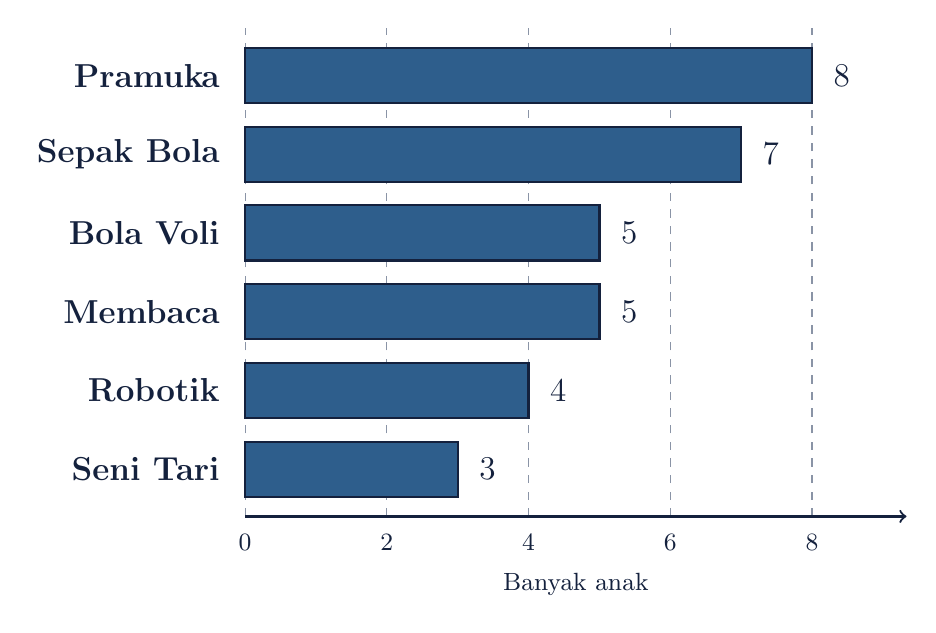
\begin{tikzpicture}
  % Garis grid dan tanda sumbu, 0 sampai 8
  \foreach \x in {0,2,4,6,8} {
    \draw[abu, thin, dashed] ({\x*0.9},0.4) -- ({\x*0.9},6.6);
    \node[anchor=north, font=\small, navy]
      at ({\x*0.9},0.3) {\x};
  }
  % Batang dan label, terurut dari yang terbesar
  \foreach \kat/\nilai/\y in
    {Pramuka/8/6, Sepak Bola/7/5, Bola Voli/5/4,
     Membaca/5/3, Robotik/4/2, Seni Tari/3/1} {
    \node[anchor=east, font=\large\bfseries, navy]
      at (-0.2,\y) {\kat};
    \draw[fill=batangbiru, draw=navy, thick]
      (0,\y-0.35) rectangle ({\nilai*0.9},\y+0.35);
    \node[anchor=west, font=\large, navy]
      at ({\nilai*0.9+0.15},\y) {\nilai};
  }
  % Sumbu mendatar
  \draw[navy, thick, ->] (0,0.4) -- (8.4,0.4);
  \node[anchor=north, font=\small, navy]
    at (4.2,-0.2) {Banyak anak};
\end{tikzpicture}

% ---------------------------------------------------------------
% Gambar 2: Versi tegak yang sesak (contoh yang dihindari).
% Label panjang dimiringkan 45 derajat dan saling bertumpuk.
% ---------------------------------------------------------------
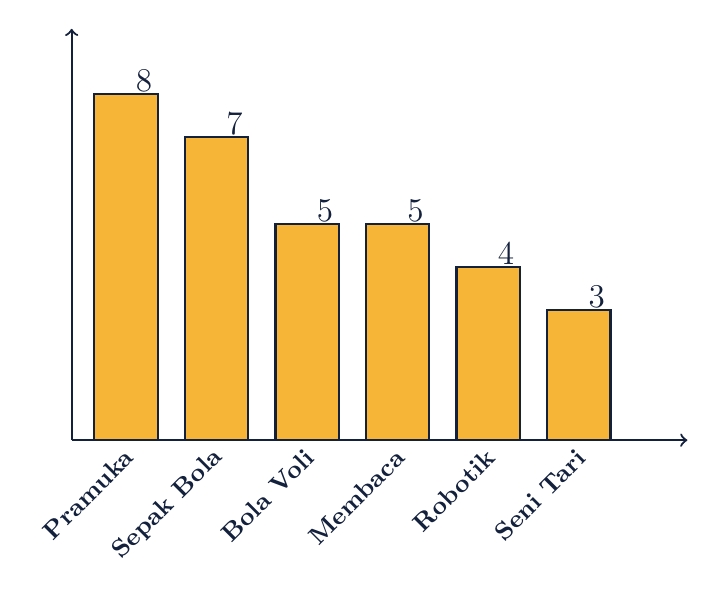
\begin{tikzpicture}[x=1.15cm, y=0.55cm]
  \foreach \kat/\nilai/\x in
    {Pramuka/8/1, Sepak Bola/7/2, Bola Voli/5/3,
     Membaca/5/4, Robotik/4/5, Seni Tari/3/6} {
    \draw[fill=batangkuning, draw=navy, thick]
      (\x-0.35,0) rectangle (\x+0.35,\nilai);
    \node[anchor=west, font=\large, navy]
      at (\x,\nilai+0.3) {\nilai};
    \node[anchor=east, rotate=45, font=\small\bfseries, navy]
      at (\x+0.1,-0.15) {\kat};
  }
  \draw[navy, thick, ->] (0.4,0) -- (0.4,9.5);
  \draw[navy, thick, ->] (0.4,0) -- (7.2,0);
\end{tikzpicture}

\end{document}
